\documentclass[a4paper]{article}
\usepackage[utf8]{inputenc}
\usepackage[russian]{babel}
\usepackage[T2]{fontenc}
\usepackage[warn]{mathtext}
\usepackage{graphicx}
\usepackage{amsmath}
\usepackage{floatflt}
\usepackage[left=20mm, top=20mm, right=20mm, bottom=20mm, footskip=10mm]{geometry}


\graphicspath{ {images/} }
\usepackage{multicol}
\setlength{\columnsep}{2cm}


\begin{document}

\begin{titlepage}
	\centering
	\vspace{5cm}
	{\scshape\LARGE Московский физико-технический институт \par}
	\vspace{4cm}
	{\scshape\Large Лабораторная работа \par}
	\vspace{1cm}
	{\huge\bfseries Закон Кюри-Вейсса \par}
	\vspace{1cm}
	\vfill
\begin{flushright}
	{\large выполнила студентка 653 группы ФФКЭ}\par
	\vspace{0.3cm}
	{\LARGE Карпова Татьяна}
\end{flushright}
	

	\vfill

% Bottom of the page
	Долгопрудный, 2017 г.
\end{titlepage}

\section{Цель работы}
Изучение температурной зависимости магнитной восприимчивости ферромагнетика выше точки Кюри

\section{В работе используются:}
\begin{itemize}
    \item катушка самоиндукции с образуом из гадолиния
    \item термостат
    \item частотомер
    \item цифровой вольтметр
    \item LC-автогенератор
    \item термопара медь-константан
\end{itemize}

\section{Теоретические положения}

При повышении температуры $T$ возрастает дезориентирующее действие теплового движения частиц, и магнитная восприимчивость ферромагнетиков убывает по закону Кюри-Вейсса
\begin{equation}
    \chi \propto \frac{1}{T - \Theta_p},
\end{equation}
где $\Theta_p$ - парамагнитная точка Кюри исследуемого вещества. При $T < \Theta_p$ образец обладает ферромагнитными свойствами и может сохранять намагниченность, при $T > \Theta_p$ образец ведёт себя как парамагнетик, для которого связь $B$ и $H$ однозначная: $I = \chi H$, $B = \mu H$. Для исследования выбран гадолиний, так как его точка Кюри лежит в интервале комнатных температур.

\section{Экспериментальная установка}

\begin{figure}[h]
    \centering
    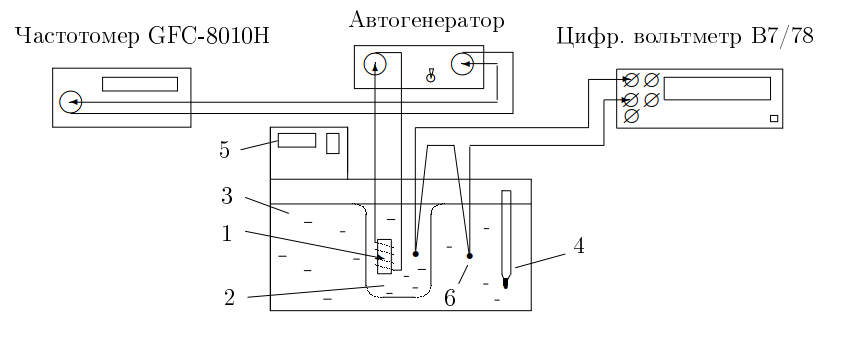
\includegraphics[width=10cm]{fig1.PNG}
    \caption{Схема экспериментальной установки}
    \label{fig:vac}
\end{figure}

Схема установки изображена на рис. 1. Исследуемый ферромагнитный образец (гадолиний) расположен внутри пустотелой катушки самоиндукции, которая служит индуктивностью колебательного контура, входящего в состав LC-автогенератора. Катушка с образцом помещена в стеклянный сосуд, залитый трансформаторным маслом. Температура образца регулируется с помощью термостата.  \par
При изменении температуры по закону Кюри-Вейсса изменяется магнитная восприимчивость образца в катушке и, следовательно, изменяется самоиндуктивность этой катушки. При этом изменяется период колебаний автогенератора. Поэтому получаем, что 
\begin{equation}
    \frac{1}{\chi} ~ (T - \Theta_p) ~ \frac{1}{(\tau^2 - \tau_0^2)},
\end{equation}
где $\tau$ и $\tau_0$ - период колебаний в цепи с сердечником в катушке и без него соответственно. Измерения проводятся в интервале температур от 14 $^{\circ}$С до 40 $^{\circ}$С

\section{Ход работы}
\begin{enumerate}
    \item Подготовим приборы к работе. Оценим допустимую ЭДС термопары: $dV = k * \triangle T = 12$ мВ, где $k = 24$град/мВ и $\triangle T = 0.5 ^{\circ}$С. Зафиксируем период колебаний контура без сердечника в катушке: $\tau_0 = 9.05$ мкс
    \item Исследуем зависимость периода колебания генератора от темературы образца, отмечая период колебаний $\tau$ по частотомеру, а температуру $T$ - по показаниям дисплея и цифровому вольтметру. Занесём в таблицу измеренные и рассчитанные значения, погрешность определения температуры по дисплею термостата $\pm 0.5^{\circ}$С, погрешность термопары составляет 12 единиц последнего разряда, получаем, что погрешность определения температуры по ней также $\pm 0.5^{\circ}$C.
    
   \begin{table}[h]
    \centering
    \begin{center}
    \caption{Зависимость периода колебаний в генераторе от температуры образца}
    \end{center}
    \vspace{0.1cm}
    \label{tab:my_label}
    \begin{tabular}{ |p{2.3cm}||p{1.2cm}|p{1.2cm}|p{1.2cm}|p{1.2cm}|p{1.2cm}|p{1.2cm}|p{1.2cm}| }
 \hline
    $T, ^{\circ}$C & 15.5 & 16.01 & 18.01 & 20 & 22 & 24 & 26 \\
\hline
    $\tau$, мкс & 10.724 & 10.703 & 10.570 & 10.320 & 9.972 & 9.611 & 9.432 \\
\hline
    $dV$, мВ & -0.002 & -0.008 & -0.019 & -0.022 & -0.022 & -0.021 & -0.021\\
\hline
    $T_{real}, ^{\circ}$C & 15.417 & 15.677 & 17.218 & 19.083 & 21.083 & 23.125 & 25.125 \\
\hline
    $\frac{1}{(\tau^2-\tau_0^2)}$, мкс$^{-2}$ & 0.030 & 0.031 & 0.034 & 0.041 & 0.057 & 0.096 & 0.142 \\
\hline
\hline
    $T, ^{\circ}$C & 28 & 30 & 32 & 34 & 36 & 38 & 40 \\
\hline
    $\tau$, мкс & 9.342 & 9.288 & 9.252 & 9.226 & 9.206 & 9.190 & 9.178 \\
\hline
    $dV$, мВ & -0.020 & -0.018 & -0.017 & -0.018 & -0.017 & -0.016 & -0.016\\
\hline
    $T_{real}, ^{\circ}$C & 27.167 & 29.250 & 31.292 & 33.250 & 35.292 & 37.333 & 39.333 \\
\hline
    $\frac{1}{(\tau^2-\tau_0^2)}$, мкс$^{-2}$ & 0.186 & 0.229 & 0.270 & 0.311 & 0.351 & 0.392 & 0.429 \\
\hline
\hline    
       \end{tabular}
\end{table}

\item Построим график зависимости $\frac{1}{(\tau^2-\tau_0^2)} = f(T)$. Прямую ферромагнитного участка экстраполируем к оси абсцисс, полученное значение - экспериментальное значение точки Кюри для исследуемого образца. 

\begin{figure}[h]
    \centering
    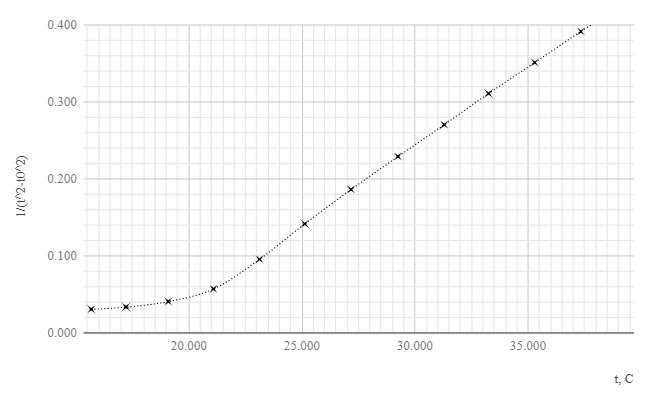
\includegraphics[width=\textwidth]{graph1.PNG}
    \caption{Зависимость $\frac{1}{(\tau^2-\tau_0^2)} = f(T)$}
    \label{fig:vac}
\end{figure}

\item Получаем значение точки Кюри гадолиния $\Theta_p = 18.6 \pm 0.7 ^{\circ}$C. Табличное значение этой величины составляет $19^{\circ}$ по данным ru.wikipedia.org/wiki/ТочкаКюри и megabook.ru/article/Гадолиний. 
\end{enumerate}

\section{Вывод}

В ходе работы была экспериментально определена парамагнитная точка Кюри для гадолиния, исследован переход его от ферромагнитного к парамагнитному состоянию. Значение точки Кюри совпало со справочным значением:
\begin{center}
    $\Theta_t_h = 19^{\circ}$C \hspace{1cm} $\Theta_e_x = 18.6 \pm 0.7^{\circ}$C
\end{center}
Можно сделать вывод, что данный метод можно использовать для веществ, у которых точка Кюри находится в интервале комнатных температур. Для других веществ можно, например, в качестве среды в термостате использовать нагретый до нужных температур пар.
\end{document}
